\documentclass[12pt,]{article}
\usepackage[compact]{titlesec}
\usepackage{fancyhdr}
\usepackage{hanging}
\pagestyle{fancy}
\usepackage{lmodern}
\usepackage{amssymb,amsmath}
\usepackage{ifxetex,ifluatex}
\usepackage{fixltx2e} % provides \textsubscript
\ifnum 0\ifxetex 1\fi\ifluatex 1\fi=0 % if pdftex
  \usepackage[T1]{fontenc}
  \usepackage[utf8]{inputenc}
\else % if luatex or xelatex
  \ifxetex
    \usepackage{mathspec}
    \usepackage{xltxtra,xunicode}
  \else
    \usepackage{fontspec}
  \fi
  \defaultfontfeatures{Mapping=tex-text,Scale=MatchLowercase}
  \newcommand{\euro}{€}
\fi
% use upquote if available, for straight quotes in verbatim environments
\IfFileExists{upquote.sty}{\usepackage{upquote}}{}
% use microtype if available
\IfFileExists{microtype.sty}{%
\usepackage{microtype}
\UseMicrotypeSet[protrusion]{basicmath} % disable protrusion for tt fonts
}{}
\usepackage{setspace}
\usepackage{lineno}
\linenumbers
\usepackage{setspace}
\usepackage{geometry}
\usepackage{ifthen}
\geometry{verbose,letterpaper,tmargin=2.54cm, bmargin=2.54cm,lmargin=2.54cm,rmargin=2.54cm}
\usepackage{graphicx}
\makeatletter
\def\maxwidth{\ifdim\Gin@nat@width>\linewidth\linewidth\else\Gin@nat@width\fi}
\def\maxheight{\ifdim\Gin@nat@height>\textheight\textheight\else\Gin@nat@height\fi}
\makeatother
% Scale images if necessary, so that they will not overflow the page
% margins by default, and it is still possible to overwrite the defaults
% using explicit options in \includegraphics[width, height, ...]{}
\setkeys{Gin}{width=\maxwidth,height=\maxheight,keepaspectratio}
\ifxetex
  \usepackage[setpagesize=false, % page size defined by xetex
              unicode=false, % unicode breaks when used with xetex
              xetex]{hyperref}
\else
  \usepackage[unicode=true]{hyperref}
\fi
\hypersetup{breaklinks=true,
            bookmarks=true,
            pdfauthor={David J. Harris},
            pdftitle={Estimating species interactions in large, abiotically structured communities with Markov networks and stochastic approximation},
            colorlinks=true,
            citecolor=blue,
            urlcolor=blue,
            linkcolor=magenta,
            pdfborder={0 0 0}}
\urlstyle{same}  % don't use monospace font for urls
\setlength{\parindent}{0pt}
\setlength{\parskip}{4pt}
\setlength{\emergencystretch}{3em}  % prevent overfull lines
\setcounter{secnumdepth}{0}

\title{Estimating species interactions in large, abiotically structured
communities with Markov networks and stochastic approximation}
\author{David J. Harris}
\date{}

\begin{document}
\maketitle


\begin{spacing}{1.9}
\begin{flushleft}
\section{Abstract}\label{abstract}

Species interactions are believed to play an important role in community
structure, but detecting their influence in the co-occurrence patterns
of observed communities has stymied ecologists for decades. While Markov
networks (undirected graphical models also known as Markov random
fields) represent a promising approach to this long-standing problem by
isolating direct interactions from indirect ones, the methods ecologists
have suggested for fitting these models are limited to small communities
with about 20 species or fewer. Additionally, the methods that have been
proposed so far do not account for environmental heterogeneity, and thus
attempt to explain all of the co-occurrence patterns in ecological data
sets with species interactions. In this paper, I introduce stochastic
approximation as an alternative method for fitting these models that
addresses both of these problems, making it feasible to use Markov
networksin cases where each species responds to multiple abiotic factors
and hundreds of competitors or mutualists. While stochastic
approximation does introduce some sampling noise during the optimization
process, it still converges to the maximum likelihood estimate for
species' interaction coefficients with probability one.

\section{Introduction}\label{introduction}

To the extent that species interactions are important for community
assembly, ecologists generally expect them to leave a signature on
species' co-occurrence patterns. Using that signature to infer the
underlying species interactions from observational data has been much
harder, however. Disagreements about how to draw these inferences led to
an acrimonious, decade-long argument among community ecologists (Lewin
1983), where essentially all of the proposed statistical approaches were
criticized for having high error rates, a poor match with the underlying
ecological questions, computational infeasibility, or all three (Connor
and Simberloff 1979, Gilpin and Diamond 1982, Strong et al. 1984,
Hastings 1987). As documented below, ecologists have, for the most part,
not solved these problems in the ensuing decades. Resolving these issues
would solve a longstanding issue in community ecology and make a
significant contribution to other fields, such as species distribution
modeling (Kissling et al. 2012).

During the time that ecologists have struggled to identify the
interactions among dozens of species, bioinformaticians have largely
solved the analogous problem of estimating interactions among thousands
of genes from their co-expression levels (e.g. Friedman et al. (2008)).
The discrepancy is due to the fact that ecologists have chosen to focus,
almost exclusively, on overall co-occurrence rates (Connor and
Simberloff 1979, Gilpin and Diamond 1982, Gotelli and Ulrich 2009, Veech
2013) or on closely-related values such as correlation coefficients
(Pollock et al. 2014; see Faisal et al. 2010 and Harris 2015 for two
recent exceptions). As ecologists know, however, the correlation between
two species will often reflect other factors beyond their direct
pairwise interactions (e.g.~abiotic influences and indirect biotic
effects; Figure 1). When these factors are not accounted for, this
reliance on overall co-occurrence rates can reliably lead to incorrect
inferences (Harris 2015a). While some methods have been proposed for
incorporating a small number of specific factors (such as geographic or
environmental dissimilarity) into ecologists' null models at a time
(Lessard et al. 2011), we still lack a good way to scale these
approaches up for cases with many biotic and abiotic factors acting
simultaneously.

\begin{figure}[htbp]
\centering
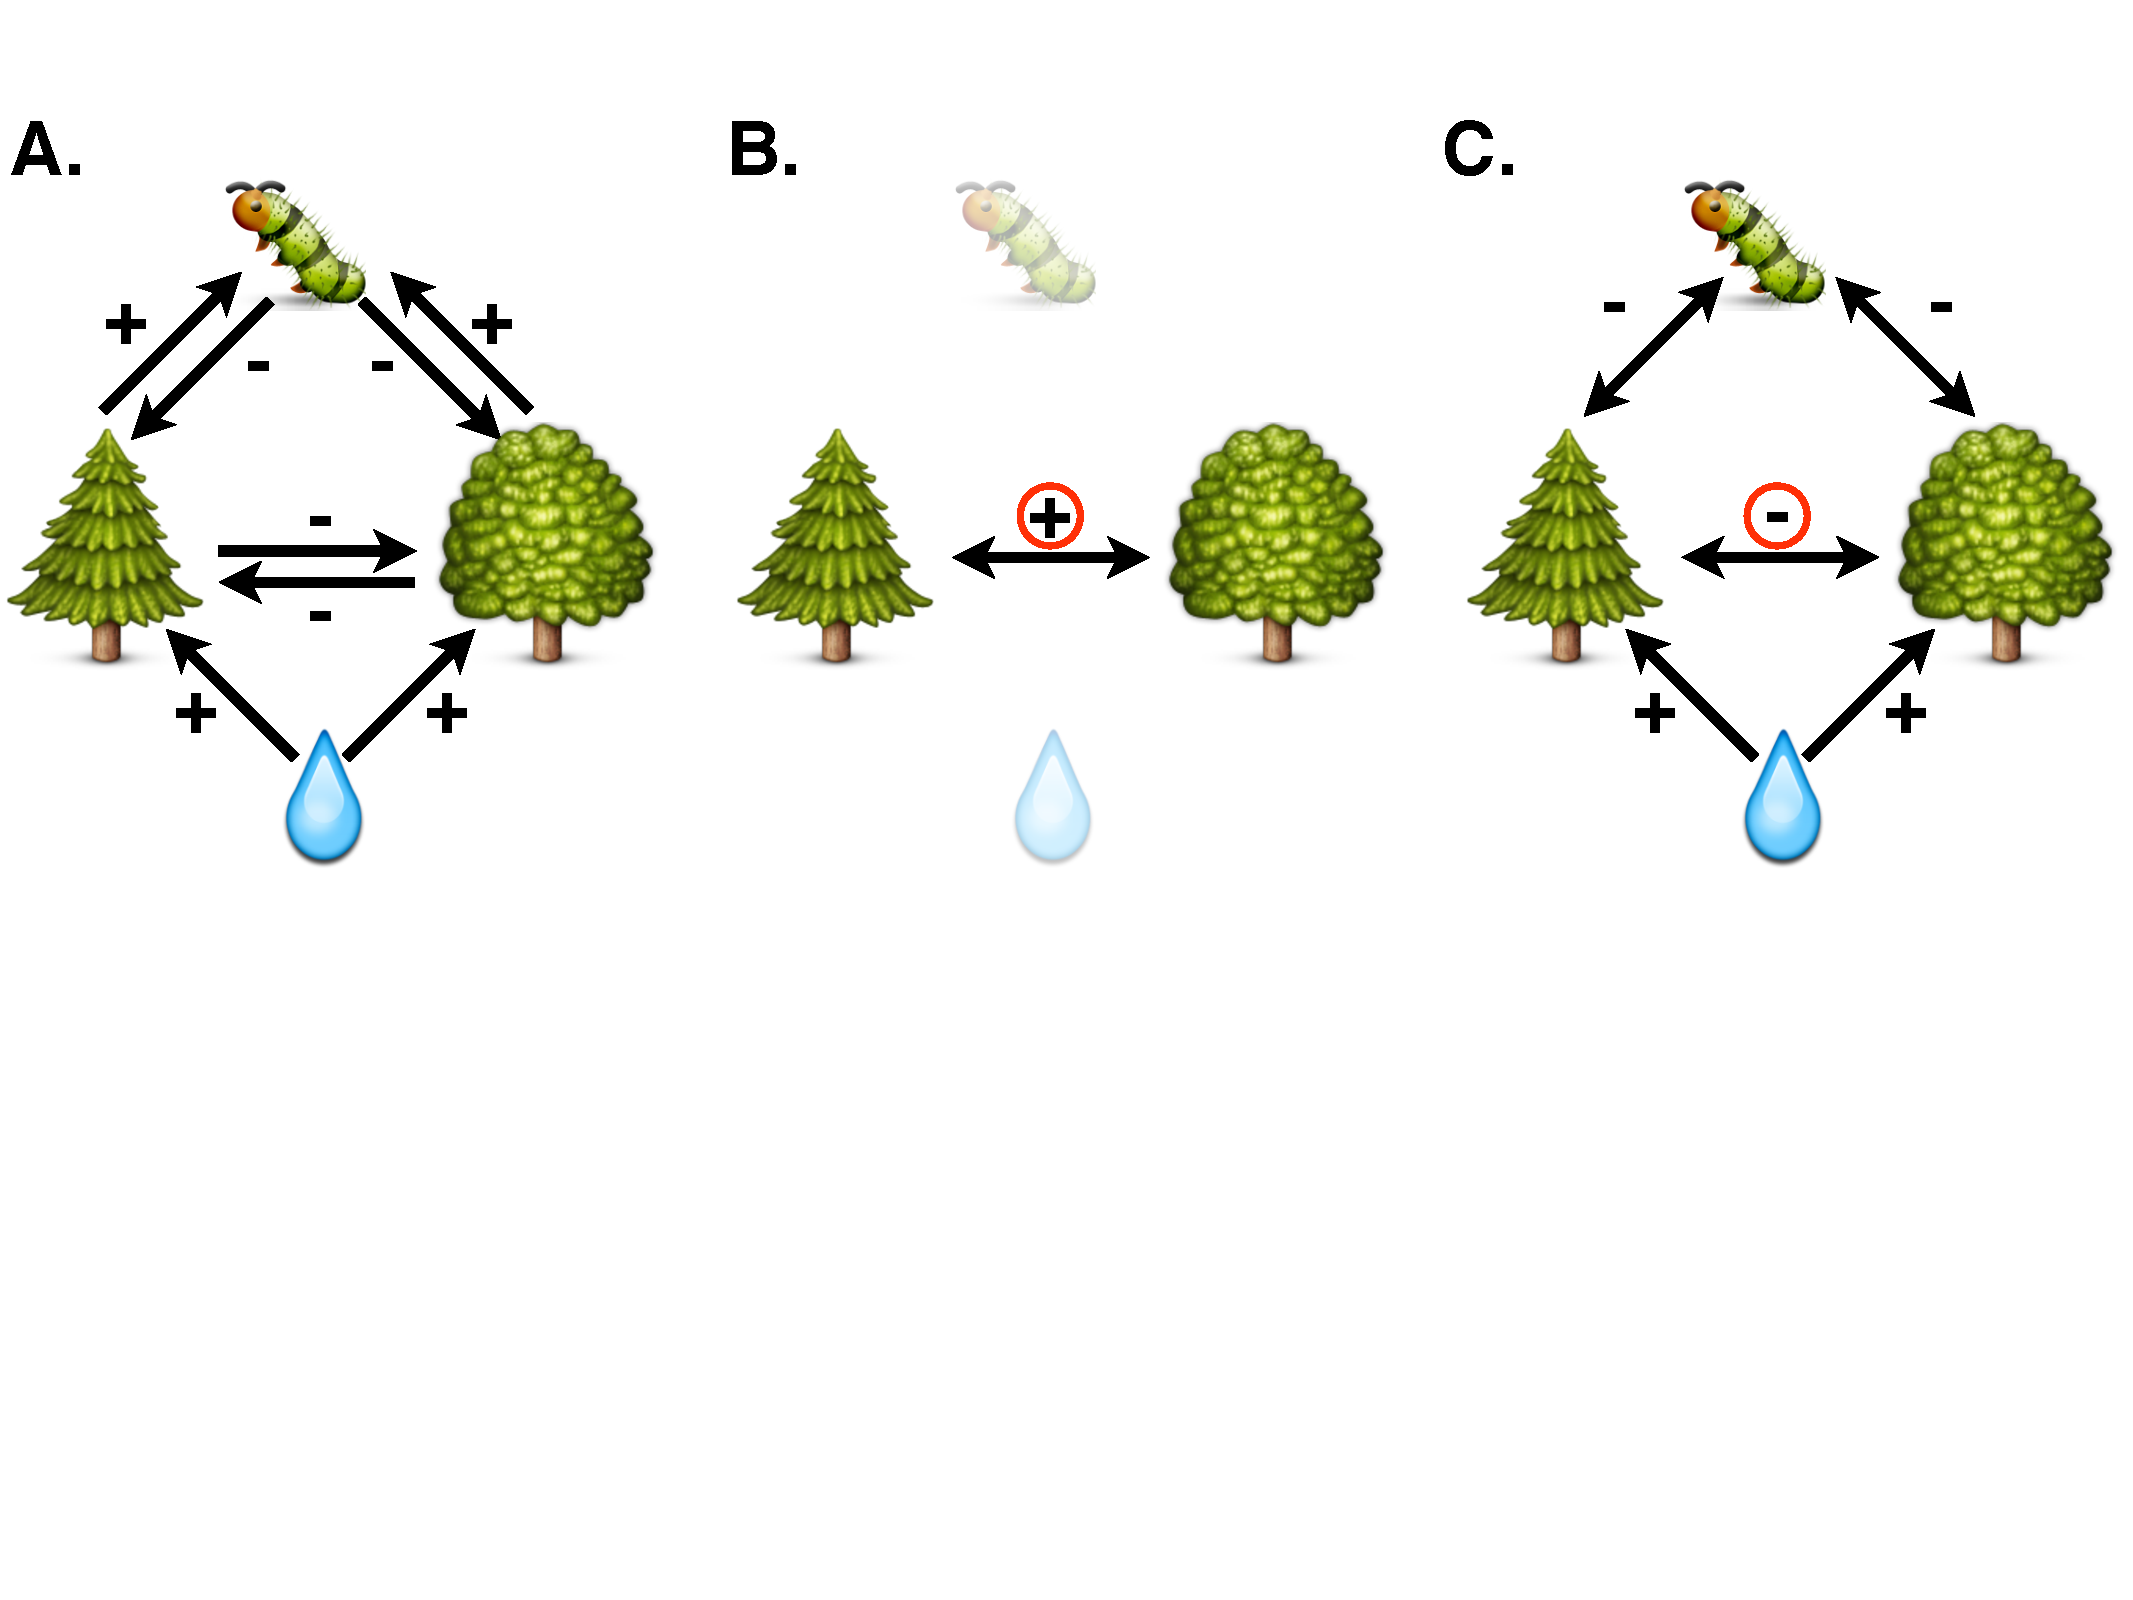
\includegraphics{figure-1.pdf}
\caption{A hypothetical network of three species, two of which depend on
an abiotic factor (annual rainfall). \textbf{A.} The ``true'' network
involves the caterpillar exploiting the two tree species as well as
competition between the two trees. The two trees also benefit from
rainfall. \textbf{B.} Although the two trees directly reduce one
another's occurrence probabilities via competition, they tend to occur
in the same areas (with sufficient water and without too many
herbivores). An analysis that ignores these other factors could
mistakenly conclude that the two trees were mutualists because of their
high co-occurrence rate (circled ``+'' sign). \textbf{C.} The methods
presented here are designed to estimate the direct interactions between
each pair of species, after accounting for other species and abiotic
factors that could affect their co-occurrence rates (note that the
circled interaction between the trees has the correct sign). Note that,
with observational data, the bi-directional effects of species
interactions (pairs of arrows between species) need to be collapsed to a
single number describing the conditional relationship between species
(one double-headed arrow).}
\end{figure}

A number of procedures have been developed for controlling for the
influence of extraneous factors and focusing on the direct relationship
between a single pair of variables, i.e.~for estimating the conditional
relationship between them. The most familiar of these is the partial
correlation. Rather than describing the overall relationship between two
variables across all conditions, partial correlations (like regression
coefficients) describe the portion of the relationship that remains
after the other variables in the data have been accounted for. Harris
(2015a) found that the partial correlation can do extract accurate
information about pairwise species interactions from binary
co-occurrence data in some circumstances, but the fact that this
approach assumes multivariate Gaussian data makes it less appealing.

Recently, several papers have suggested that ecologists could use Markov
networks (undirected graphical models also known as Markov random
fields) to estimate conditional relationships from binary data by
maximum entropy or maximum likelihood (Azaele et al. (2010); Harris
(2015a)). A Markov network defines a probability distribution over
possible binary species assemblages, and its coefficients (including one
coefficient describing the conditional relationship between each pair of
species in the network). This approach is optimal in the sense that it
produces a model that matches the observed properties of the data
(i.e.~the occurrence and co-occurrence rates), and that it does so with
the fewest possible parameters or constraints (i.e.~the Markov network
has the most information entropy of any possible model satisfying its
constraints; Azaele et al. 2010). As shown in Harris (2015a), Markov
networks do a better job of estimating species' influences on one
another better than a number of existing methods, particularly when
sample sizes are low.

Unfortunately, Markov networks have an intractable likelihood function
whose computational difficulty more than doubles each time a new species
is added to the model. This exponential growth in the likelihood
function's complexity means that the methods that worked for Azaele et
al. (2010) and Harris (2015a) with networks of 20 species would be
completely infeasible for networks with 50 species, requiring over a
billion times more computational effort
(\(2^{50}/2^{20} \approx 10^{9}\)). Extending the method to account for
abiotic variation among sites on the landscape would require repeating
these expensive computations independently for every site, increasing
the computational burden even further. If ecologists want to apply these
methods to larger problems, a different model-fitting algorithm would be
needed.

In this paper, I present a different way of optimizing the likelihood,
called ``stochastic approximation'' (Robbins and Monro 1951,
Salakhutdinov and Hinton 2012), which replaces the intractable
computations with tractable Monte Carlo estimates of the same
quantities. Despite the sampling error introduced by this substitution,
stochastic approximation provides strong guarantees for eventual
convergence to the maximum likelihood estimate (Younes 1999,
Salakhutdinov and Hinton 2012). This change in approach makes it
feasible to estimate the interactions among hundreds of species from
observational data while also accounting for possible responses to
abiotic factors (such as those used in species distribution models),
giving ecologists some power to distinguish between species pairs that
co-occur due to shared environmental tolerances from those that co-occur
due to direct interactions like mutualism.

\section{Methods}\label{methods}

\subsection{Markov networks}\label{markov-networks}

As discussed in Azaele et al. (2010) and Harris (2015a), Markov networks
such as the Ising model (Cipra 1987) can be used to describe community
structure as follows. Each species is represented by a binary random
variable, describing whether it is present (1) or absent (0). A species'
conditional probability of presence under a given set of biotic and
abiotic conditions depends on its coefficients. The coefficients linking
species to one another describe their conditional associations: all else
equal, a species will occur less often in the presence of its
competitors and other species with which it is negatively associated,
and more often in the presence of its mutualists:

\[ p(y_i | \vec{y}_{j \neq i}) = \mathrm{logistic}\Big(\alpha_i + \sum_{j \neq i}{\beta_{ij}y_j}\Big), \]

where \(y_i\) is 1 when species \(i\) is present and 0 when it is
absent, \(\alpha_i\) is an intercept term, \(\beta_ij\) represents the
conditional relationship between species \(i\) and species \(j\), and
\(\mathrm{logistic}(x) = e^x / (1 + e^x)\). These conditional
probabilities can be combined to calculate the probability of observing
any given combination of presences and absences, up to a multiplicative
constant (Lee and Hastie 2012, Murphy 2012):

\[p(\vec{y}) \propto \mathrm{exp}\Big({\sum_{i}{\alpha_i y_i} + \sum_{j \neq i}}{\beta_{ij} y_i y_j}\Big).\]

Unfortunately, the exponentially large number of possible assemblages
makes the normalizing constant for this joint probability distribution
intractable when the number of species is larger than 20 or so. However,
it is generally straightforward to simulate examples of assemblages that
are consistent with graphical models such as these, using Monte Carlo
techniques like Gibbs sampling (Salakhutdinov and Hinton 2012). Gibbs
sampling is especially convenient for these models because it only
requires the conditional probabilities, which are straightforward to
compute (Harris 2015; Appendix).

In each of the scenarios below, the ``observed'' landscapes were
simulated using Gibbs sampling from a pre-specified set of ``true''
parameters, then stochastic approximation was used to recover these
parameters from the simulated presence-absence data.

\subsection{Conditioning the network on the abiotic
environment}\label{conditioning-the-network-on-the-abiotic-environment}

The Markov networks fit in Harris (2015a) treated the \(\alpha_i\) terms
from Equations 1 and 2 as constants, meaning that the models expected
each species to have the same conditional occurrence probability in any
location with a given set of facilitators and competitors. In this
paper, I extend the model so that the local abiotic conditions can also
affect species occurrence probabilities directly. Specifically, the
\(\alpha_i\) terms in these analyses are linear combinations of the
local environmental conditions, represented by \(x_1\) through \(x_5\).
By estimating the coefficients associated with each of these \(x\)
variables for each species, we can account for their responses to the
abiotic environment as well as to one another. In other fields, a model
like this one, where a Markov network's parameters depend on external
factors is called a conditional random field (Lee and Hastie 2012);
these models have been used in a variety of contexts, from language
models to image processing (Murphy 2012).

\subsection{Coefficient estimation with stochastic
approximation}\label{coefficient-estimation-with-stochastic-approximation}

A Markov network describes a probability distribution over possible
assemblages. Since the model is a member of the exponential family it
can be summarized without loss of information by its ``sufficient
statistics''. For the model presented here, the sufficient statistics
include: the number of occurrences for each species, the number of
co-occurrences between each species, and the cross-product between the
species and environment matrices (Azaele et al. 2010, Lee and Hastie
2012, Murphy 2012). Finding the maximum likelihood estimate for the
model parameters is equivalent to minimizing the discrepancy between the
values of the data's sufficient statistics and the expected sufficient
statistics under the model (Bickel and Doksum 1977). Because
fully-observed Markov networks, such as the ones analyzed here, have
unimodal likelihood functions (Murphy 2012), it is possible to find the
global optimum by iteratively reducing the discrepancies between the
sufficient statistics of the model and of the data to zero.

In order to reduce the discrepancy between the observed and predicted
sufficient statistics, the \texttt{rosalia} calculates each value
exactly, averaging over all possible presence-absence combinations.
Stochastic approximation (Robbins and Monro 1951, Salakhutdinov and
Hinton 2012) instead estimates the expected values of the sufficient
statistics by averaging over a more manageable number of simulated
assemblages during each model-fitting iteration, while still retaining
maximum likelihood convergence guarantees. The procedure iterates
through the following three steps as many times as needed (50,000 for
these analyses; see Appendix for annotated R code):

\begin{enumerate}
\def\labelenumi{\arabic{enumi}.}
\item
  Simulate a set of assemblages from the current model parameters and
  calculate sufficient statistics for the sample.
\item
  Subtract the simulated sufficient statistics from the observed ones to
  calculate the approximate likelihood gradient
\item
  Adjust the model parameters to climb the approximate gradient, using a
  schedule of step sizes that satisfies the criteria in Chapter 6 of
  Powell (2007).
\end{enumerate}

Here, the simulations in Step 1 used Gibbs sampling to generate examples
of landscapes based on the model's current parameter estimates. While
the simulated landscapes produced by Gibbs sampling are serially
autocorrelated, statisticians have shown that this merely slows
convergence to the maximum likelihood estimate rather than preventing it
altogether (Younes 1999, Salakhutdinov and Hinton 2012).

The approximate likelihood gradients in Step 2 match the ones from
Harris (2015a), except that they are averaged over a set of Monte Carlo
samples rather than over all possible presence-absence combinations.
These gradients were augmented with a momentum term (Hinton 2012) and by
regularizers based on a logistic prior with location 0 and scale 2.0
(for environmental responses) or 0.5 (for pairwise interactions). The
step size parameter in Step 3, \(\alpha_t\), decreased after each
iteration according to a generalized harmonic sequence,
\(\alpha_t = 1000/(999 + t)\), which satisfies the criteria in Powell
(2007).

\subsection{Simulated landscapes with known
interactions}\label{simulated-landscapes-with-known-interactions}

In order to assess the models' ability to recover the ``true''
parameters that generated a presence-absence matrix of interest, I first
needed to generate such matrices from known processes.

To demonstrate that my stochastic approximation implementation could
converge to the global optimum, I first simulated a landscape with 20
species and 500 sites, using Gibbs sampling. These landscapes had few
enough species that the \texttt{rosalia} package for estimating Markov
networks (Harris 2015b) could find the penalized maximum likelihood
estimates for the Markov network in a reasonable amount of time. For
each of these simulated landscapes, I then fit the same Markov network
model to the simulated data using the exact approach from Harris (2015a)
and the stochastic approximation method described above.

I then simulated a large landscape with 250 species and 2500 sites,
representing a large data set roughly the size of the North American
Breeding Bird Survey. Each site on the landscape was represented by 5
environmental variables, which were drawn independently from Gaussian
distributions with mean 0 and standard deviation 2.5.

Each species was assigned two sets of coefficients. The coefficients
determining species' responses to the environment were each drawn from
standard normal distributions. The coefficients describing species'
pairwise interactions were drawn from a mixture of normals (see
Appendix) so that most interactions were weak and negative, but a few
strong positive and interactions also occurred.

The coefficients described above are sufficient to define each species'
conditional occurrence probability (i.e.~its probability of occurrence
against any given backdrop of biotic and abiotic features). I used these
conditional probabilities to produce examples of communities that were
consistent with the competition parameters and with the local
environmental variables via Markov chain Monte Carlo (specifically, 1000
rounds of Gibbs sampling; see code in the Appendix). I then used the
methods from the next section to attempt to infer the underlying
parameters from the simulated data.

\section{Results}\label{results}

\begin{figure}[htbp]
\centering
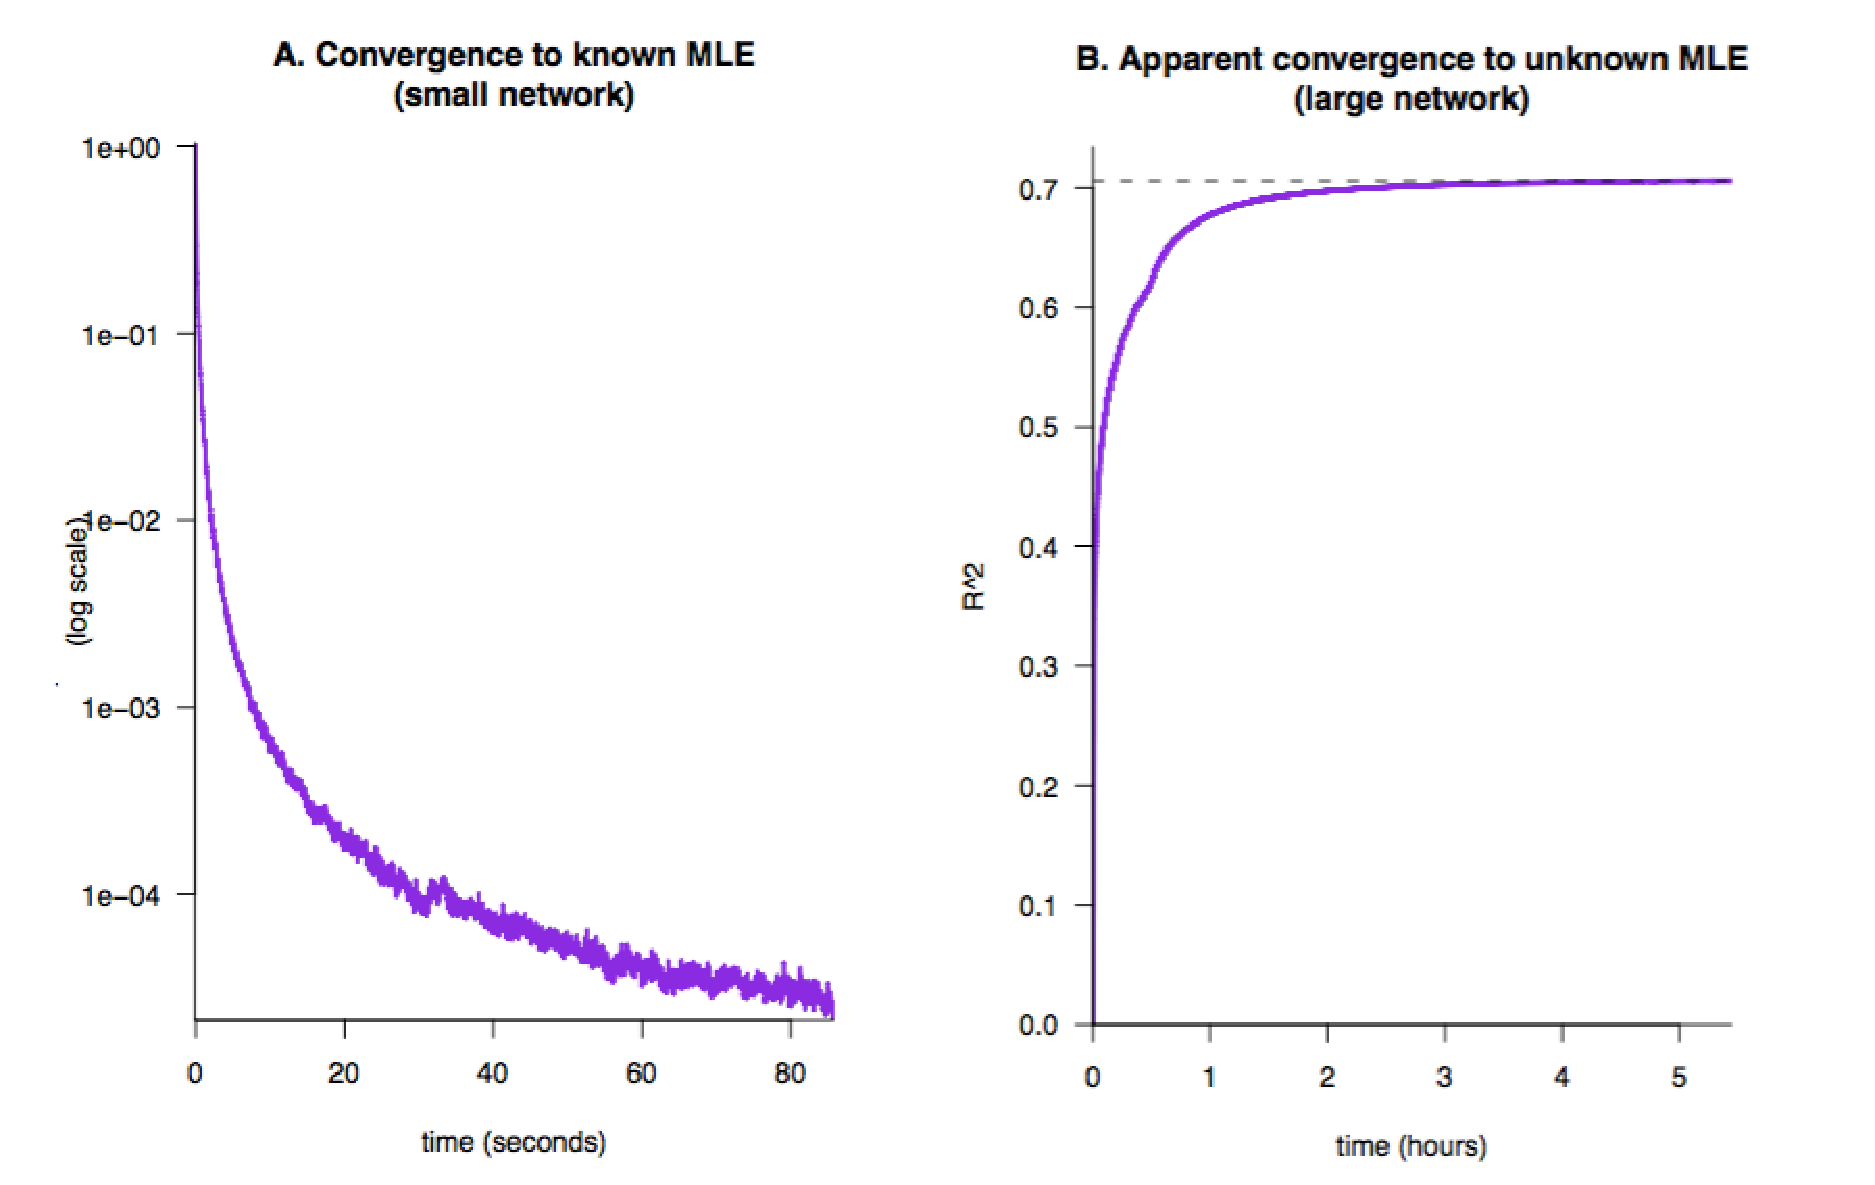
\includegraphics{convergence.pdf}
\caption{Stochastic approximation improves the model over time.
\textbf{A.} With small networks where the exact maximum likelihood
estimates are known, stochastic approximation approaches the global
optimum very quickly (note the log scale of the y axis). Within a few
seconds, the mean squared deviation between the approximate and exact
estimates drops to less than 0.01; in less than a minute, it drops below
0.0001. For comparison, the \texttt{rosalia} package took about six
minutes to find the maximum likelihood estimate. \textbf{B.} With larger
networks, where the maximum likelihood estimate cannot be calculated
exactly, stochastic approximation converges to an apparent optimum that
explains most (but not all) of the variation in the ``true'' parameter
values.}
\end{figure}

For the smaller communities, the squared deviations between the exact
estimates produced by the \texttt{rosalia} package and the ones produced
by stochastic approximation quickly decayed to negligible levels (Figure
2A), indicating that the stochastic approximation procedure was
implemented correctly and worked as the mathematical theory predicts.

\begin{figure}[htbp]
\centering
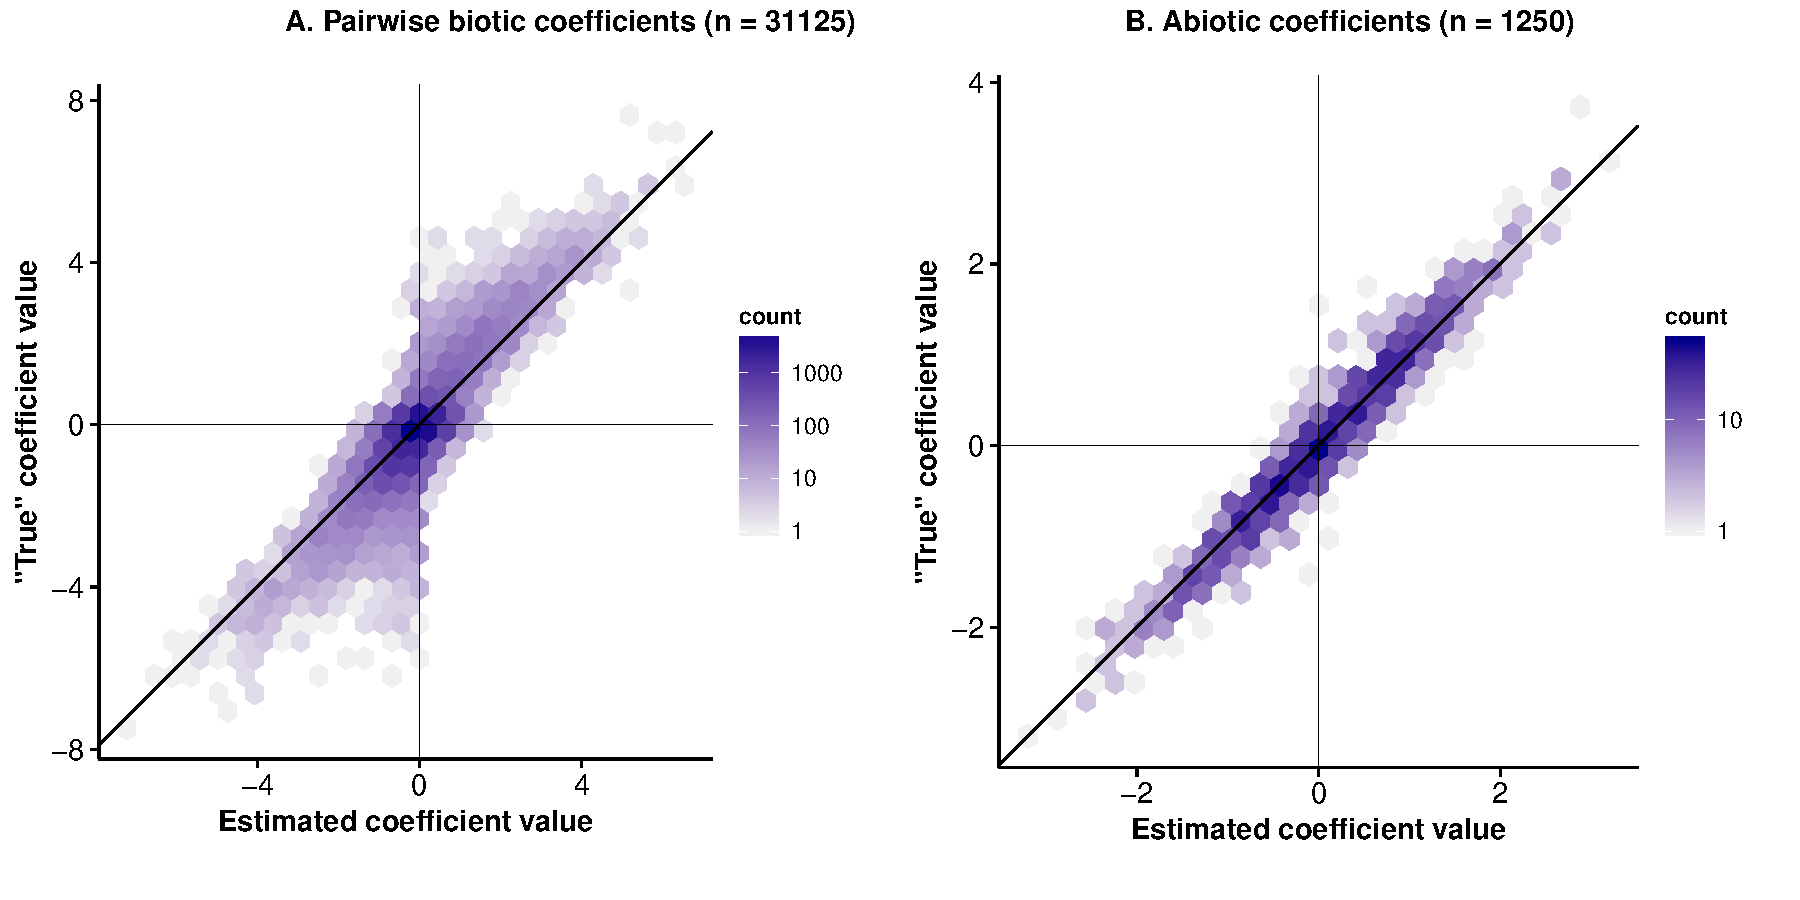
\includegraphics{estimates.pdf}
\caption{``True'' versus estimated network parameters for all 250
species' responses to the other 249 species in the data set (\textbf{A.}
\(R^2 = .71\)) and to the 5 abiotic variables (\textbf{B.}
\(R^2 = .95\)).}
\end{figure}

For the larger landscape, I found that the stochastic approximation
approach achieved reasonably good performance after ten minutes of
optimization (Figure 2B). After 50,000 iterations (about 5.4 hours on my
laptop), the model was able to recover more than two thirds of the
variance in species' pairwise interactions(\(R^2 = 0.71\); Figure 3A),
and nearly all of the variance in their responses to environmental
variables (\(R^2 = 0.95\); Figure 3B).

\section{Discussion}\label{discussion}

For decades, ecologists have relied on poor test statistics for
inferring species interactions from observational data (Harris 2015a).
As shown here and in Harris (2015a), however, these inferences can only
be made reliably by methods that control for other species in the
network, such as partial correlations or Markov networks. The biggest
computational problem with large Markov networks is the impossibility of
averaging over all their possible states, but these results demonstrate
that this step can be avoided in ecological analyses. Stochastic
approximation is able to recover the same estimates as exact methods for
smaller networks, while scaling gracefully to networks with hundreds of
species.

The largest downside of using stochastic approximation instead of the
exact methods introduced in Harris (2015a) is the difficulty in
generating confidence intervals. The \texttt{rosalia} package can
produce confidence intervals based on the Hessian matrix, but it is not
feasible to calculate this matrix for large networks. It may turn out
that the best way to generate confidence intervals for large networks is
by repeatedly fitting the model to bootstrapped samples of the data.
Alternatively, ecologists may be able to take advantage of the advanced
Monte Carlo techniques introduced in Murray et al. (2012) to sample from
the posterior distribution over possible parameter values, which could
be used to generate credible intervals for the parameter estimates.
Other advanced Monte Carlo methods (e.g. Salakhutdinov 2009) may also
speed up convergence to the maximum likelihood estimate in cases where
serial autocorrelation in the Gibbs sampler is too strong for
effectively sampling the space of possible landscapes.

As the number of potentially-interacting species increases, the number
of adjustable parameters increases even faster, so overfitting becomes a
major concern. Fortunately, a number of good regularizers have been
proposed. Of these, some of the most interesting options include \(L_1\)
regularization, which ensures that many of the estimated coefficients
are exactly zero (Lee and Hastie 2012). This sparsity matches
ecologists' intuition that many species from different guilds are
unlikely to interact much at all (Faisal et al. 2010), and also produces
computational benefits for model estimation. Of course, the best
regularizers will take advantage of specific ecological knowledge
(e.g.~from field experiments, natural history, or trait data) to provide
information about individual pairwise interactions, rather than about
their overall distribution.

These richer sources of information will be especially important for
cases where ecologists expect that the interactions between species are
asymmetric (e.g.~where only one species is affected by an interaction or
where one species benefits at a cost to the other). With snapshot
observations of species' spatial associations, as discussed here,
interactions must be reduced to a single number describing the net
association, as in undirected models such as the Markov networks
presented here (Schmidt and Murphy 2012). With richer data types,
however, ecologists could more easily learn about asymmetric
interactions such as facilitation, predation, and parasitism.

Even without better data, ecologists have a number of options for
expanding beyond simple Markov networks in a number of ways that would
improve their ability to address a wider range of questions. This paper
demonstrated that it is possible to simultaneously estimate species'
responses to the abiotic and environment and to one another, but many
other extensions are possible. For example, ecologists could condition
the model on variables whose values have not been measured
(e.g.~partially-observed Markov networks, or the approximate networks in
the \texttt{mistnet} package; cf. Pollock et al. (2014)). This would
allow ecologists to account for measurement error and for other
ecologically-important factors that can be difficult to measure.
Ecologists should also explore higher-order networks, where one species'
presence can affect the relationship between two other species (Whittam
and Siegel-Causey 1981, Tjelmeland and Besag 1998).

\section*{References}\label{references}
\addcontentsline{toc}{section}{References}

\hyperdef{}{refs}{\label{refs}}
\hyperdef{}{ref-azaeleux5finferringux5f2010}{\label{ref-azaeleux5finferringux5f2010}}
Azaele, S., R. Muneepeerakul, A. Rinaldo, and I. Rodriguez-Iturbe. 2010.
Inferring plant ecosystem organization from species occurrences. Journal
of theoretical biology 262:323--329.

\hyperdef{}{ref-bickelux5fmathematicalux5f1977}{\label{ref-bickelux5fmathematicalux5f1977}}
Bickel, P., and K. Doksum. 1977. Mathematical Statistics: Basic Ideas
and Selected Topics. San Francisco: Holden---Day.

\hyperdef{}{ref-cipraux5fintroductionux5f1987}{\label{ref-cipraux5fintroductionux5f1987}}
Cipra, B. A. 1987. An introduction to the Ising model. American
Mathematical Monthly 94:937--959.

\hyperdef{}{ref-connorux5fassemblyux5f1979}{\label{ref-connorux5fassemblyux5f1979}}
Connor, E. F., and D. Simberloff. 1979. The assembly of species
communities: Chance or competition? Ecology:1132--1140.

\hyperdef{}{ref-faisalux5finferringux5f2010}{\label{ref-faisalux5finferringux5f2010}}
Faisal, A., F. Dondelinger, D. Husmeier, and C. M. Beale. 2010.
Inferring species interaction networks from species abundance data: A
comparative evaluation of various statistical and machine learning
methods. Ecological Informatics 5:451--464.

\hyperdef{}{ref-friedmanux5fsparseux5f2008}{\label{ref-friedmanux5fsparseux5f2008}}
Friedman, J., T. Hastie, and R. Tibshirani. 2008. Sparse inverse
covariance estimation with the graphical lasso. Biostatistics
9:432--441.

\hyperdef{}{ref-gilpinux5ffactorsux5f1982}{\label{ref-gilpinux5ffactorsux5f1982}}
Gilpin, M. E., and J. M. Diamond. 1982. Factors contributing to
non-randomness in species Co-occurrences on Islands. Oecologia
52:75--84.

\hyperdef{}{ref-gotelliux5fempiricalux5f2009}{\label{ref-gotelliux5fempiricalux5f2009}}
Gotelli, N. J., and W. Ulrich. 2009. The empirical Bayes approach as a
tool to identify non-random species associations. Oecologia
162:463--477.

\hyperdef{}{ref-harrisux5festimatingux5f2015}{\label{ref-harrisux5festimatingux5f2015}}
Harris, D. J. 2015a. Estimating species interactions from observational
data with Markov networks. bioRxiv.

\hyperdef{}{ref-harrisux5frosaliaux5f2015}{\label{ref-harrisux5frosaliaux5f2015}}
Harris, D. J. 2015b. Rosalia: Exact inference for small binary Markov
networks. R package version 0.1.0. Zenodo.
http://dx.doi.org/10.5281/zenodo.17808.

\hyperdef{}{ref-hastingsux5fcanux5f1987}{\label{ref-hastingsux5fcanux5f1987}}
Hastings, A. 1987. Can competition be detected using species
co-occurrence data? Ecology:117--123.

\hyperdef{}{ref-hintonux5fpracticalux5f2012}{\label{ref-hintonux5fpracticalux5f2012}}
Hinton, G. E. 2012. A practical guide to training restricted boltzmann
machines. Pages 599--619 \emph{in} Neural Networks: Tricks of the Trade.
Springer.

\hyperdef{}{ref-kisslingux5ftowardsux5f2012}{\label{ref-kisslingux5ftowardsux5f2012}}
Kissling, W. D., C. F. Dormann, J. Groeneveld, T. Hickler, I. Kühn, G.
J. McInerny, J. M. Montoya, C. Römermann, K. Schiffers, F. M. Schurr, A.
Singer, J.-C. Svenning, N. E. Zimmermann, and R. B. O'Hara. 2012.
Towards novel approaches to modelling biotic interactions in
multispecies assemblages at large spatial extents. Journal of
Biogeography 39:2163--2178.

\hyperdef{}{ref-leeux5flearningux5f2012}{\label{ref-leeux5flearningux5f2012}}
Lee, J. D., and T. J. Hastie. 2012, May. Learning Mixed Graphical
Models.

\hyperdef{}{ref-lessardux5fstrongux5f2011}{\label{ref-lessardux5fstrongux5f2011}}
Lessard, J.-P., M. K. Borregaard, J. A. Fordyce, C. Rahbek, M. D.
Weiser, R. R. Dunn, and N. J. Sanders. 2011. Strong influence of
regional species pools on continent-wide structuring of local
communities. Proceedings of the Royal Society of London B: Biological
Sciences.

\hyperdef{}{ref-lewinux5fsantaux5f1983}{\label{ref-lewinux5fsantaux5f1983}}
Lewin, R. 1983. Santa Rosalia Was a Goat. Science 221:636--639.

\hyperdef{}{ref-murphyux5fmachineux5f2012}{\label{ref-murphyux5fmachineux5f2012}}
Murphy, K. P. 2012. Machine Learning: A Probabilistic Perspective. The
MIT Press.

\hyperdef{}{ref-murrayux5fmcmcux5f2012}{\label{ref-murrayux5fmcmcux5f2012}}
Murray, I., Z. Ghahramani, and D. MacKay. 2012. MCMC for
doubly-intractable distributions. arXiv preprint arXiv:1206.6848.

\hyperdef{}{ref-pollockux5funderstandingux5f2014}{\label{ref-pollockux5funderstandingux5f2014}}
Pollock, L. J., R. Tingley, W. K. Morris, N. Golding, R. B. O'Hara, K.
M. Parris, P. A. Vesk, and M. A. McCarthy. 2014. Understanding
co-occurrence by modelling species simultaneously with a Joint Species
Distribution Model (JSDM). Methods in Ecology and Evolution:n/a--n/a.

\hyperdef{}{ref-powellux5fapproximateux5f2007}{\label{ref-powellux5fapproximateux5f2007}}
Powell, W. B. 2007. Approximate Dynamic Programming: Solving the curses
of dimensionality. John Wiley \& Sons.

\hyperdef{}{ref-robbinsux5fstochasticux5f1951}{\label{ref-robbinsux5fstochasticux5f1951}}
Robbins, H., and S. Monro. 1951. A Stochastic Approximation Method. The
Annals of Mathematical Statistics 22:400--407.

\hyperdef{}{ref-salakhutdinovux5flearningux5f2009}{\label{ref-salakhutdinovux5flearningux5f2009}}
Salakhutdinov, R. 2009. Learning in Markov random fields using tempered
transitions. Advances in neural information processing systems
22:1598--1606.

\hyperdef{}{ref-salakhutdinovux5fefficientux5f2012}{\label{ref-salakhutdinovux5fefficientux5f2012}}
Salakhutdinov, R., and G. Hinton. 2012. An efficient learning procedure
for deep Boltzmann machines. Neural Computation 24:1967--2006.

\hyperdef{}{ref-schmidtux5fmodelingux5f2012}{\label{ref-schmidtux5fmodelingux5f2012}}
Schmidt, M., and K. Murphy. 2012. Modeling Discrete Interventional Data
using Directed Cyclic Graphical Models. arXiv preprint arXiv:1205.2617.

\hyperdef{}{ref-strongux5fecologicalux5f1984}{\label{ref-strongux5fecologicalux5f1984}}
Strong, D. R., D. Simberloff, L. G. Abele, and A. B. Thistle. 1984.
Ecological communities: Conceptual issues and the evidence. Princeton
University Press.

\hyperdef{}{ref-tjelmelandux5fmarkovux5f1998}{\label{ref-tjelmelandux5fmarkovux5f1998}}
Tjelmeland, H., and J. Besag. 1998. Markov Random Fields with
Higher-order Interactions. Scandinavian Journal of Statistics
25:415--433.

\hyperdef{}{ref-veechux5fprobabilisticux5f2013}{\label{ref-veechux5fprobabilisticux5f2013}}
Veech, J. A. 2013. A probabilistic model for analysing species
co-occurrence. Global Ecology and Biogeography 22:252--260.

\hyperdef{}{ref-whittamux5fspeciesux5f1981}{\label{ref-whittamux5fspeciesux5f1981}}
Whittam, T. S., and D. Siegel-Causey. 1981. Species Interactions and
Community Structure in Alaskan Seabird Colonies. Ecology 62:1515--1524.

\hyperdef{}{ref-younesux5fconvergenceux5f1999}{\label{ref-younesux5fconvergenceux5f1999}}
Younes, L. 1999. On the convergence of Markovian stochastic algorithms
with rapidly decreasing ergodicity rates. Stochastics: An International
Journal of Probability and Stochastic Processes 65:177--228.
\end{flushleft}
\end{spacing}

\end{document}
